% ProofAlign anonymous NDSS 2027 submission source.
\documentclass[conference]{IEEEtran}

\usepackage{graphicx}
\usepackage{cite}
\usepackage{mathtools}
% NDSS requires a Times-family face; load newtx after amsmath/mathtools so the
% text and mathematics fonts remain portable across Tectonic and Overleaf.
\usepackage{newtxtext,newtxmath}
\usepackage{textcomp}
\usepackage{xcolor}
\usepackage{xspace}
\usepackage{array}
\usepackage{tabularx}
\usepackage{placeins}
\usepackage{booktabs}
\usepackage{tikz}
\usepackage{url}
\usepackage[hidelinks]{hyperref}
\usetikzlibrary{positioning,arrows.meta,fit,shapes.geometric,patterns}
\Urlmuskip=0mu plus 1mu

\pagestyle{plain}
\hyphenation{op-tical net-works semi-conduc-tor Action-Block}

\begin{document}

\title{ProofAlign: Trusted-Task Monitoring and Cross-Layer Execution Integrity for Action-Only Vision--Language--Action Systems}

% Double-blind submission.
\author{}

% Required NDSS 2027 first-page publication block.  Replace the placeholder
% when the submission system assigns the Fall-cycle paper number.
\IEEEoverridecommandlockouts
\makeatletter\def\@IEEEpubidpullup{6.5\baselineskip}\makeatother
\IEEEpubid{\parbox{\columnwidth}{
  Network and Distributed System Security (NDSS) Symposium 2027\\
  22--26 March 2027, Seoul, Republic of Korea\\
  ISBN 978-1-970672-09-1\\
  https://dx.doi.org/10.14722/ndss.2027.24xxxx\\
  www.ndss-symposium.org
}
\hspace{\columnsep}\makebox[\columnwidth]{}}

\maketitle

\newcommand{\system}{\textsc{ProofAlign}\xspace}
\newcommand{\actionblock}{\textsc{ActionBlock}\xspace}
\newcommand{\lone}{\textsc{L1}\xspace}
\newcommand{\ltwoa}{\textsc{L2a}\xspace}
\newcommand{\ltwob}{\textsc{L2b}\xspace}
\newcommand{\dual}{\textsc{Dual}\xspace}

\begin{abstract}
Vision--language--action (VLA) systems map language and multimodal observations
to continuous robot actions.  At deployment, an online action chunk crosses
from model output into the execution stack without inherent evidence that it
is admissible for the current task, that later software preserves it, or that
its realization is qualified for the current robot state.  Existing defenses
typically stop at model input or candidate selection, or begin from an already
trusted command, program, or reference trajectory.

We present \system, an inline consumer-side reference monitor that makes the
exact source \actionblock the protected object.  Under an explicit trusted-task
and observation assumption, \lone attaches a checker-relative assessment to
the block.  \ltwoa carries its identity through a fresh one-use authorization,
ordered dispatch, receipts, effects, and task-phase advance.  When a registered
joint boundary triggers, \ltwob qualifies at most two temporary virtual-guard
configurations without changing or resampling the source action.  We formalize
the composition as $\mathsf{ProofAligned}$---checker-relative eligibility,
transaction alignment, and conditional containment---and use Lean to
machine-check its finite authorization, ordered-action, receipt, evidence, and
phase-transition relations.

Using SABER on a complete 120-unit attack-evaluation protocol, we measure 39 of
86 clean-eligible units as new risk transitions (45.35\%, 95\% base-pair
cluster-bootstrap CI: [32.93\%, 57.78\%]).  A separate paired four-arm study
contains 18 task/initialization pairs and 144 episodes.  Under attack, VLA-only
and L2-only succeed on 11/18 tasks, whereas L1-only and Dual succeed on 13/18;
their joint-limit violation-episode counts are 4/18, 1/18, 0/18, and 0/18.
Screening reaches 39.79\,ms maximum and 18.30\,ms p95, with no 100\,ms miss.
The empirical studies run in LIBERO-Safety simulation; they support the stated
checker-relative and transaction properties for the evaluated configuration,
not complete semantic correctness, hardware attestation, hard-real-time
behavior, or general robot safety.
\end{abstract}

\IEEEpeerreviewmaketitle

\section{Introduction}
\label{sec:introduction}

Vision--language--action (\vla) models are moving robot control from fixed task
programs toward policies that translate language and multimodal observations
directly into continuous actions~\cite{pi05,rth2024}.  In the action-only
interface studied here,
each policy call returns an ordered \actionblock to a consumer, which dispatches
the block and then replans from a new observation.  This block is the first
concrete object that leaves the learned policy and becomes eligible for physical
execution; it is therefore a natural security boundary
(Figure~\ref{fig:motivation}).

\begin{figure}[!t]
\centering
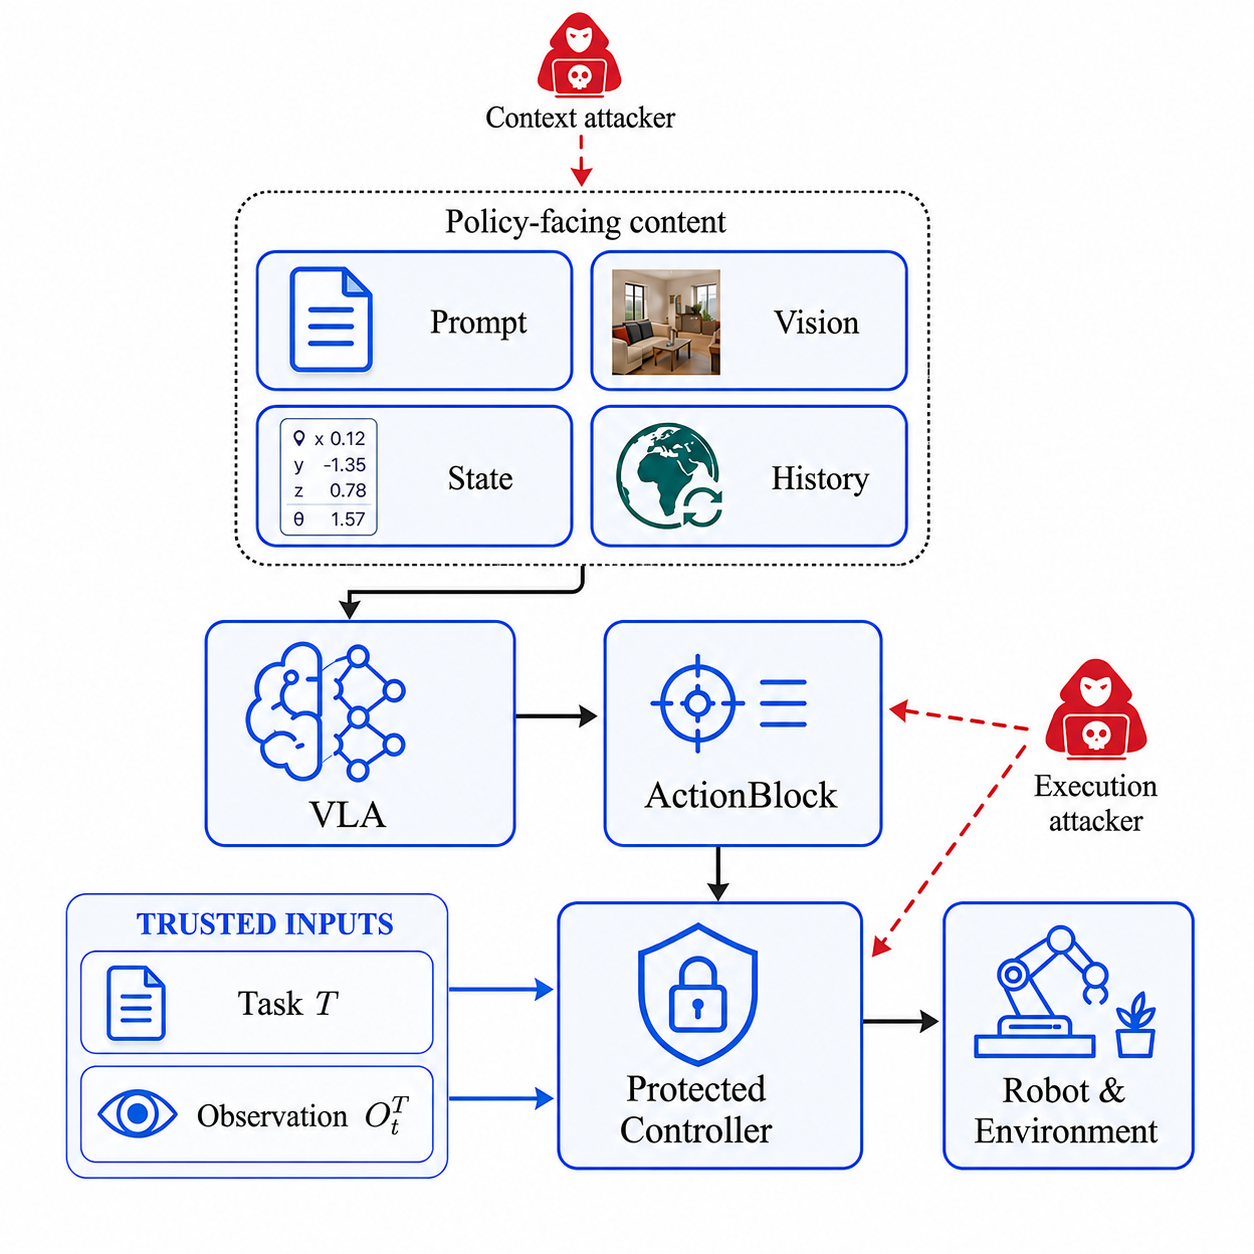
\includegraphics[width=.98\columnwidth]{figures/motivation_boundary_raster_v2_square.png}
\caption{Deployment and protection overview.  Attacks may corrupt policy inputs
or tamper with post-inference execution.  \system mediates the point at which a
newly generated continuous \actionblock becomes executable.}
\label{fig:motivation}
\end{figure}

That boundary is exposed from both sides.  Instruction perturbations, visual
perturbations, and embodied-agent jailbreaks can change the action produced by a
\vla~\cite{saber2026,freezevla2025,badrobot2025,robopair2025}.  In the motivating
SABER case, the authoritative task is to move a soda can to a plate, while the
policy is induced to act on ``move to the farthest fixture.''  The consumer sees
only the resulting numeric block, not a trustworthy account of which task
authorized it.  After inference, compromised software can additionally replace
the proposal, replay an earlier permission, reorder steps, or splice evidence
from different proposals~\cite{diat2019,cfaplus2024,arto2026,tat2026}.  An input
attack and an execution attack thus meet at the same actuator-facing object.

Existing defenses protect important parts of this path.  Structured-input and
trusted-agent architectures protect instruction/data separation or derive
digital control flow from a trusted query~\cite{struq2025,secalign2025,
camel2026,ace2026}.  Action attribution and trajectory auditing explain tool
calls or mobile-agent behavior~\cite{attriguard2026,mate2026}.  \vla verifiers
assess plan--action consistency or learned alignment over action candidates
~\cite{sealvla2026,covervla2026}.  CPS integrity and robot-attestation systems
bind protected programs, reference motion, or control flow to execution
evidence~\cite{diat2019,cfaplus2024,arto2026,tat2026}; prediction and shielding
qualify candidate consequences or continuous safety sets
~\cite{vlmpc2024,safetychance2024,measurementrobustcbf2021,
realizableshields2025}.

These defenses stop at different points around the online \actionblock.  Input
and agent defenses do not establish that the block later accepted by the robot
is the one justified by trusted task state.  Candidate verifiers may rank or
score a policy proposal, but do not preserve that verdict through ordered
dispatch and observed effects.  Execution-integrity systems begin from a
protected program or previously specified motion, while shields qualify a
physical constraint without connecting the decision back to task-relative
authority.  The surveyed defense families therefore protect different segments
of the path.  Their stated mechanisms do not jointly bind independently anchored
task authority to the exact newly generated block, its ordered dispatch, and
registered execution evidence.

This missing composition exposes two alignment gaps.  The \emph{intent--action
authorization gap} lies between trusted task intent and the exact \actionblock
generated from an attackable policy view.  The \emph{action--execution
realization gap} lies between an admitted block and its ordered dispatch,
evidence, and state-dependent physical realization.  C1 belongs to the first
stage.  C2 and C3 are the transaction-integrity and guarded-realization
obligations within the second stage.

The core question is how an action-only consumer can establish
checker-relative task authorization for an exact source block and preserve that
authorization through qualified execution without modifying the \vla.

The key insight is to treat the exact online \actionblock as the stable identity
anchor across the entire lifecycle.  Evidence attaches to this observable
object, avoiding assumptions about the model's latent intent or a unique
reference trajectory.  A scoped task-relative assessment names the source
block, the same proposal persists through dispatch and effect evidence, and any
state-dependent execution configuration is recorded separately.  Physical
qualification therefore cannot silently change the object named by earlier
evidence.

Turning this insight into a runtime monitor raises three challenges.  \textbf{C1
concerns semantic assessment.}  A task phase may admit many valid trajectories,
so the monitor must distinguish covered hard risks from uncertain task progress
without presenting a local checker as a complete semantic oracle.  \textbf{C2
concerns execution identity.}  Assessment, permission, ordered dispatch,
receipts, and effects must remain attached to one proposal and one state epoch
under replay and reordering attempts.  \textbf{C3 concerns state-dependent
realization.}  Near a physical boundary, the monitor must qualify an execution
configuration while keeping the policy's source action fixed and making failure
explicit.

\system realizes this two-stage design as an inline consumer-side reference
monitor~\cite{saltzer1975,schneider2000}.  \lone aligns trusted task intent with
the exact source \actionblock through checker-relative \taskassessment (C1).
Covered hard risks reject before dispatch; task-progress uncertainty remains
advisory.  \ltwo aligns the admitted source block with execution.  Its
\transactionbinding component (\ltwoa) binds the proposal to a one-use ordered
transaction and requires matching receipts and effects (C2).
\guardscreening (\ltwob) qualifies the same source action under a registered
joint-boundary trigger before dispatch (C3).  Together, the two stages implement
the \proofaligned lifecycle property while leaving the \vla checkpoint,
policy-facing prompt, and single-source-block generation unchanged.

The threat and the final system are evaluated in two deliberately separate
studies.  The attack-reproduction study pairs clean and SABER-attacked rollouts
for 120 seed-specific units and measures whether an attack creates a new
physical-risk transition.  The system study reruns the same population under
clean and attacked conditions for 960 attempts.  Its four paired arms are
\vlaonly, \loneonly, \ltwoonly, and \dual.  This design separates the reproduced
ASR from the four-arm mechanism comparison and reports task success independently
from physical-risk outcomes.

The attack reproduction yields an observed ASR of 45.35\% among 86
clean-eligible units (39/86).  In the separate four-arm study, the common
75-unit cohort has broad risk-transition rates of 50.67\%, 56.00\%, 48.00\%,
and 57.33\%; the paired sensitivity tests provide no evidence of a broad
reduction.  Each condition has 98.96\% valid traces (475/480), leaving the
registered all-valid dependency unmet and the comparisons nonconfirmatory.
Under attack, \dual task success is 53.33\%, compared with 60.83\% for
\vlaonly.  The narrower registered joint-side result covers the 237 valid
attacked \ltwoenabled traces.  None contains a joint-limit step (0.00\%), while
valid attacked \vlaonly and \loneonly traces contain 4,960 and 2,452 such
steps.  This supports the targeted guard property within its validity boundary;
it is not a general robot-safety claim.

All claims are checker-relative and TCB-relative.  The empirical scope is one
$\pi_{0.5}$ checkpoint, LIBERO-Safety simulation, and one frozen SABER
instruction-attack family.

This work makes three contributions.
\begin{itemize}
  \item \textbf{A protected object and lifecycle security property.}  This work
  identifies the exact online \actionblock as the common object across
  task-relative assessment, execution identity, and state-conditioned
  realization, and defines the adversary, TCB, evidence endpoints, and
  \proofaligned property.
  \item \textbf{A two-stage cross-layer reference monitor.}  \system composes
  \lone intent--action assessment with \ltwo action--execution transaction and
  guard enforcement while keeping source-action identity fixed.  Lean checks
  selected abstract transaction and phase relations.
  \item \textbf{An attack reproduction and paired system characterization.}
  The evaluation quantifies the reproduced SABER attack, compares the final
  system and its two stage ablations, and reports broad risk, task success,
  targeted joint-side behavior, invalid traces, and runtime cost without merging
  their distinct estimands.
\end{itemize}

\section{Background and Motivation}
\label{sec:background}

\subsection{The Action-Only Execution Boundary}

An embodied \vla deployment has three logical roles.  An operator or scheduler
supplies a task, a policy maps its task view and multimodal observations to a
continuous \actionblock, and a consumer sends the block to an actuator-facing
controller.  After the block is consumed, the environment supplies a new
observation and the policy replans.  The policy therefore exports neither a
trusted task proof nor a predeclared reference trajectory; it exports an ordered
numeric proposal~\cite{pi05}.

For policy call $t$, write the source block as
\begin{equation}
A_t=(a_{t,0},\ldots,a_{t,H-1})\in\mathbb{R}^{H\times d}.
\label{eq:action-block-background}
\end{equation}
The consumer must decide whether this block is admissible, ensure that its rows
reach the controller in the intended order, and interpret the effects observed
after execution.  These are different questions: a task-relative assessment
does not itself establish execution integrity, and faithful dispatch does not
itself establish a physical safety property.

\subsection{How Attacks Reach the Same Object}

SABER perturbs policy-facing instructions, FreezeVLA perturbs visual input, and
embodied-agent jailbreaks manipulate language or multimodal context
~\cite{saber2026,freezevla2025,badrobot2025,robopair2025}.  Although these attacks
enter through different modalities, their physical influence is mediated by the
online block produced at the action-only interface.  They instantiate the
\intentaction surface; RQ1 exercises the SABER instruction channel.

After inference, a software
adversary can target the same lifecycle by substituting the source block,
reordering or omitting steps, replaying an earlier permission, or attaching
receipts and effects from a different proposal
~\cite{diat2019,cfaplus2024,arto2026,tat2026}.  These faults target the
\actionexecution transaction path enforced by \ltwoa.

The meaning of an accepted source action also depends on state and execution
configuration.  The same controller input can realize differently as joint
margins, contacts, or controller constraints change
~\cite{vlmpc2024,safetychance2024,measurementrobustcbf2021,
realizableshields2025}.  This state-dependent realization risk is the registered
target of \ltwob and need not arise from a separate attacker action.  The
security question spans the path from task authority, through the generated
block, to ordered execution and state-conditioned physical realization.

\subsection{Where Existing Protection Boundaries Stop}

Upstream defenses establish trusted inputs, protected digital control flow, or
an assessment over one or more policy candidates
~\cite{struq2025,secalign2025,camel2026,ace2026,sealvla2026,covervla2026}.
Their evidence ends before the full actuator transaction.  Execution-side
systems establish integrity for protected programs, control flow, or reference
motion~\cite{diat2019,cfaplus2024,arto2026,scaphy2023,tat2026}; their authority
begins from an already specified program or trajectory.  Prediction and
shielding qualify possible consequences or a local safety set, but do not by
themselves connect that decision to an independently anchored task assessment of
the newly generated block.

Table~\ref{tab:capability-comparison} summarizes these stopping points using
the six capabilities that define the protected lifecycle in this paper.

\begin{table*}[t]
\centering
\caption{Capability coverage across adjacent defenses at the action-only
boundary.  For a family row, a check means that at least one cited member states
a mechanism matching the column; a cross marks a capability outside the row's
stated endpoint.  The symbols do not rank overall system strength.}
\label{tab:capability-comparison}
\footnotesize
\setlength{\tabcolsep}{3.4pt}
\renewcommand{\arraystretch}{1.15}
\begin{tabularx}{\textwidth}{>{\raggedright\arraybackslash}X*{6}{>{\centering\arraybackslash}p{0.096\textwidth}}}
\toprule
Work family & \shortstack{Trusted/\\untrusted\\authority split}
  & \shortstack{Task--action\\assessment}
  & \shortstack{Exact action\\identity}
  & \shortstack{Receipt/effect\\binding}
  & \shortstack{Physical\\qualification}
  & \shortstack{Formal/\\attested\\semantics} \\
\midrule
StruQ, SecAlign~\cite{struq2025,secalign2025}
  & \pacovered & \panotcovered & \panotcovered & \panotcovered & \panotcovered & \panotcovered \\
AttriGuard~\cite{attriguard2026}
  & \pacovered & \pacovered & \pacovered & \panotcovered & \panotcovered & \panotcovered \\
CaMeL, ACE~\cite{camel2026,ace2026}
  & \pacovered & \pacovered & \pacovered & \panotcovered & \panotcovered & \pacovered \\
SEAL, CoVer~\cite{sealvla2026,covervla2026}
  & \panotcovered & \pacovered & \panotcovered & \panotcovered & \panotcovered & \panotcovered \\
DIAT, CFA+, ARTO, SCAPHY~\cite{diat2019,cfaplus2024,arto2026,scaphy2023}
  & \pacovered & \panotcovered & \panotcovered & \pacovered & \pacovered & \pacovered \\
TAT~\cite{tat2026}
  & \pacovered & \panotcovered & \panotcovered & \pacovered & \pacovered & \pacovered \\
Prediction and shielding~\cite{vlmpc2024,safetychance2024,measurementrobustcbf2021,realizableshields2025}
  & \panotcovered & \pacovered & \panotcovered & \panotcovered & \pacovered & \pacovered \\
\textbf{\system}
  & \pacovered & \pacovered & \pacovered & \pacovered & \pacovered & \pacovered \\
\bottomrule
\end{tabularx}
\end{table*}

The missing composition is therefore a proposal-scoped lifecycle with two
stages.  The first links authoritative task state to assessment of the source
block.  The second links an admitted block to ordered dispatch, receipts, and
effects, with an additional qualification obligation when robot state approaches
the registered boundary.  Section~\ref{sec:related} gives the detailed
comparison.  These stopping points yield the design requirements below.

\subsection{Three Design Challenges}

\textbf{C1. Bind semantic authority to a continuous proposal.}
A task phase can admit many valid continuous trajectories, so a monitor cannot
simply compare the policy output with one reference motion.  It needs an
independently anchored description of the current legal subtask and a checker
whose verdict states exactly which properties it covers.  Covered hard risks
must block execution, while uncertain task progress must not be presented as a
complete semantic guarantee.

\textbf{C2. Preserve proposal identity through execution.}
An assessment is useful only if later permission, dispatch, receipts, effects,
and task-phase advance refer to the same proposal and observation epoch.  The
consumer must reject substitution, replay, reordering, partial evidence, and
cross-proposal splicing while ensuring that failed evidence cannot be mistaken
for successful completion.

\textbf{C3. Qualify state-dependent realization without changing the source
action.}
Near a physical boundary, the controller configuration may need to change how a
source action is realized.  The design must keep the policy-produced row fixed,
make the selected guard/controller configuration explicit, and qualify that
combination before dispatch.  ``Same action'' therefore means the same policy
output at the protected controller boundary, not an assertion that every
controller configuration produces an identical physical trajectory.

\begin{table}[t]
\centering
\caption{The two alignment stages and their three component obligations.}
\label{tab:challenges}
\footnotesize
\begin{tabularx}{\columnwidth}{l>{\raggedright\arraybackslash}Xl}
\toprule
Component & Required invariant & Stage \\
\midrule
\lone (C1) & Verdict names the source block and checker scope & I \\
\ltwoa (C2) & Permission, dispatch, receipts, and effects share one proposal & II \\
\ltwob (C3) & Qualification names the fixed source action and configuration & II \\
\bottomrule
\end{tabularx}
\end{table}

The next section turns these challenges into an adversary model, trusted
assumptions, and lifecycle security objective.  Section~\ref{sec:design} then
presents the three corresponding components within the two stages.

\section{Problem Definition and Threat Model}
\label{sec:model}

We model an ordinary embodied VLA policy call and define the evidence required
before its output may affect task state.  The formulation is independent of the
evaluation platform; Section~\ref{sec:evaluation} later instantiates it in
LIBERO-Safety.

\subsection{System Model and Protected Object}

Let $x_t$ denote the embodied system state at epoch $t$, $T$ an authoritative
task artifact, and $O_t^T$ the observation used by the monitor.  The VLA
receives a policy view $(P_t^{pol},O_t^{pol},H_t^{pol})$ containing its prompt,
observation, and history.  These views may agree during nominal execution or
diverge after input corruption.  Their separation is a TCB assumption: logging
policy-facing bytes does not make those bytes authoritative.

At state epoch $t$, the two branches compute
\begin{equation}
\begin{aligned}
Z_t &= \mathsf{SelectFrozen}(T,O_t^T),\\
A_t &= \pi(P_t^{pol},O_t^{pol},H_t^{pol}),\\
S_t &= \mathsf{AssessLocal}(Z_t,O_t^T,A_t).
\end{aligned}
\end{equation}
$Z_t$ is selected and frozen before the policy returns $A_t$.  It is an
independent monitor anchor, not a recovered latent intent or a hidden prompt to
the policy.  The compiler maps $T$ to a trusted task graph
$\mathcal G_T=(V_T,E_T,\ell_T,\Phi_T)$: vertices are legal task phases, edges
are permitted phase transitions, $\ell_T$ gives each vertex a canonical
skill/entity tuple, and $\Phi_T(O_t^T)\subseteq V_T$ is the state-enabled
frontier.  \textsf{SelectFrozen} may emit $Z_t=\ell_T(v_t)$ only for
$v_t\in\Phi_T(O_t^T)$; otherwise it emits \texttt{unknown}.  The graph encodes
semantic authority, not a reference trajectory.  In deployment, $T$ could be a
signed job ticket or protected workflow state.  Without an independent task
source, \system cannot create authority and its semantic claim does not apply.

The protected object is the exact online block
$A_t\in\mathbb{R}^{H\times d}$, represented by its ordered numeric values and
shape in the runtime's canonical domain.  Assessment $S_t$ binds $A_t$ to
$(Z_t,O_t^T)$.  The consumer then creates execution contract $C_t$, one-use
authorization $\mathit{Auth}_t$, ordered receipts $R_t$, and effect evidence
$E_t$; $g_t$ denotes the selected execution configuration.  Every object binds
the episode nonce, proposal index, and state epoch; changes invalidate reuse.
The command identity denotes equality in a canonical numeric domain, not raw
memory equality or a guaranteed physical trajectory.  The executable identity
is at least $(A_t,g_t,t)$ because the same numeric block can realize differently
under a different controller or guard configuration.

\subsection{Attack Path and Adversary}

The adversary controls inputs and software outside the TCB.  Its path begins
after the secure split: it may modify the policy-facing instruction,
digital/software visual input, or policy history while leaving the protected
task branch unchanged.  The resulting frozen-policy call can produce a
task-divergent or risk-inducing source block.  After assessment, the adversary
may attempt command substitution, step reordering, stale-authorization replay,
cross-proposal receipt/effect splicing, or omission of unfavorable evidence.
Its objective is either to cause an unauthorized or covered-risk dispatch, or
to make a failed transaction appear eligible for task-phase advance.

This model does not assume that the policy checkpoint is malicious: a known,
immutable policy remains an untrusted proposer because its context is
attackable.  Conversely, controlling code outside the TCB does not grant the
adversary a second actuator path; complete mediation by the registered
dispatch boundary is a trusted assumption stated below.  Our empirical attack
study instantiates instruction modification, and the focused integrity suite
instantiates the modeled transaction faults.  Visual and history attacks are
in system scope but are not empirically evaluated.

\subsection{Trusted Assumptions and Evidence Endpoints}

The TCB contains the authoritative task source, trusted observation tap,
task-graph compiler and selector, local checker, contract compiler,
nonce/digest ledger, single dispatch boundary, effect observer, and protected
evidence storage.  The policy, policy-facing prompt/observation/history, and
source \actionblock are untrusted.  This is a software reference-monitor model:
we assume the TCB code and its cryptographic primitives execute as specified;
the trusted tap precedes the modeled policy-view transformation; every
actuator command traverses the single dispatch boundary; and receipt/effect
storage cannot be rewritten outside the TCB.

Three mediated endpoints delimit the evidence chain: the authority tap captures
$T$ and $O_t^T$ before policy-view modification; the dispatch boundary records
the command accepted by the actuator interface; and the effect window opens
only after dispatch.  Evidence outside these endpoints cannot establish task
authority, command application, or a post-dispatch effect, respectively.  In
particular, a policy explanation shares the attacked context, a pre-dispatch
prediction is not a receipt, and an unbound later observation is not evidence
for the current proposal.

\subsection{Proof Alignment Property}

Collect the evidence for one proposal as
$\chi_t=(T,O_t^T,Z_t,A_t,S_t,C_t,g_t,\mathit{Auth}_t,R_t,E_t)$.  We define the
top-level checker-relative property
\begin{equation}
\begin{aligned}
\mathsf{ProofAligned}(\chi_t)\triangleq {}&
\mathsf{Eligible}_t\land\mathsf{TxnAligned}_t\\
&\land(\mathsf{Triggered}_t\Rightarrow\mathsf{Contained}_t).
\end{aligned}
\label{eq:proof-aligned}
\end{equation}
The three conjuncts correspond directly to the three challenges in
Section~\ref{sec:background}.  They are defined below in terms of evidence that
the runtime can produce and check.

\textbf{P1---checker-relative eligibility.}  A block may receive covered-risk
authorization only if a qualified checker assessed that exact block against a
legal $Z_t$ and the matching trusted observation epoch.  The implemented
condition is

\begin{align}
\mathsf{Eligible}_t \triangleq {}&
  \mathsf{TrustedProv}(T,O_t^T,Z_t) \nonumber\\
&\land \mathsf{LegalFrontier}(T,O_t^T,Z_t) \nonumber\\
&\land \mathsf{Bound}(S_t,Z_t,O_t^T,A_t) \nonumber\\
&\land \mathsf{ScreenAvailable}(S_t) \nonumber\\
&\land \neg\mathsf{HardRisk}(S_t) \nonumber\\
&\land \mathsf{Qualified}(S_t.\mathit{assessor}).
\end{align}

This definition establishes provenance, frontier legality, assessment identity,
and covered hard gates.  It does not establish that every admissible action
advances $T$.  Task-progress and unavailable articulation evidence are
advisory and force next-block replanning; velocity, workspace, unexpected
contact, stale/malformed commands, and unsupported unknown evidence are hard
gates.

\textbf{P2---transaction alignment.}  A task phase may advance only if the
authorization is fresh and bound to the proposal, the dispatched prefix is
ordered and exact, and the post-dispatch evidence satisfies the contract:
\begin{align}
\mathsf{TxnAligned}_t \triangleq {}&
  \mathsf{FreshAndBound}(C_t,\mathit{Auth}_t,R_t) \nonumber\\
&\land \mathsf{OrderedExactPrefix}(R_t,\mathit{Auth}_t) \nonumber\\
&\land \mathsf{AfterDispatch}(E_t,R_t) \nonumber\\
&\land \mathsf{Required}(C_t)\subseteq E_t \nonumber\\
&\land \mathsf{Forbidden}(C_t)\cap E_t=\emptyset \nonumber\\
&\land \neg\mathsf{ObsViolation}(E_t).
\end{align}
The contract binds the action, semantic-subtask, policy-prompt, assessment, and
trusted-observation digests; state epoch; required/forbidden effects; and the
observation window.  An authorization can be consumed once.  In Python,
$\mathsf{OrderedExactPrefix}$ requires contiguous receipt indices and checks
each applied-step digest against \texttt{authorization.action\_at(i)}.  The
Lean model represents the same ordered per-step digest list and proves that
every bound receipt resolves at its index to the applied digest; Python
additionally enforces contiguous indices.  A complete serializer refinement is
outside the theorem scope.  An incomplete prefix, unknown effect, or receipt
from another proposal cannot advance the phase.

\textbf{P3---covered physical containment.}  Let $g_t$ be the selected guard
configuration and $m_j(g_t,A_t,O_t^T)$ the predicted next-step margin for joint
side $j$.  A triggered screen qualifies only when
\begin{align}
\mathsf{Contained}_t \triangleq {}&
  \mathsf{SameSource}(g_t,A_t)\land\mathsf{Restored}(g_t) \nonumber\\
&\land \min_{j\in\{1,\ldots,14\}}m_j(g_t,A_t,O_t^T)\geq0.15 \nonumber\\
&\land \mathsf{Force}(g_t,A_t,O_t^T)\leq 10{,}000.
\end{align}
The goal is covered joint-side containment, not exact trajectory reproduction
or arbitrary collision avoidance.

The distinction between source action and executable configuration is
important.  A virtual guard leaves $A_t$ unchanged but changes how the
controller maps its values to motion.  The runtime records this configuration,
but the current Lean contract does not yet type-bind it as an independent
digest.  We expose that refinement gap rather than equating command identity
with physical-trajectory identity.

Task-state progress is stricter than local acceptance.  Let $q_t$ and
$q_{t+1}$ be consecutive task phases.  The monitor enforces
\begin{equation}
\begin{aligned}
\mathsf{Advance}(q_t,q_{t+1})
&\Rightarrow \mathsf{ProofAligned}(\chi_t)\\
&\phantom{\Rightarrow{}}\land
\mathsf{CompletionObserved}(q_t,q_{t+1},E_t).
\end{aligned}
\label{eq:phase-advance}
\end{equation}
Lean mechanizes the finite identity, authorization, receipt, evidence, and
phase-transition subrelation of Eqs.~\ref{eq:proof-aligned}
and~\ref{eq:phase-advance}; task selection, checker soundness, and continuous
containment remain explicit qualification obligations.

\subsection{Out of Scope}

We exclude task-source or monitor compromise, attacks that corrupt the monitor
observation before the trusted tap, forged actuator feedback inside the TCB,
and actuator paths that bypass the mediator.  Hashes, nonces, and Lean semantics
do not supply a hardware root of trust, sensor correctness, arbitrary-dynamics
robustness, or hard-real-time guarantees.  If the trusted and policy views share
a compromised source, or the observer omits a relevant effect, a transaction
may be internally aligned yet wrong about the physical world.  The empirical
scope of the current implementation is stated separately in
Section~\ref{sec:evaluation} and Section~\ref{sec:discussion}.

\section{Design}
\label{sec:design}

\subsection{Overview}

\system is an inline consumer-side verifier, rather than a new policy or a
remote robot attestation service.  It places one trusted authority path beside
the untrusted proposal path and mediates their only route to the actuator
interface.  Figure~\ref{fig:overview} separates three system stages.  During
\emph{construction and qualification}, the monitor compiles $T$ into
$\mathcal G_T$, registers checker/effect vocabularies, and qualifies their
implementations; it does not generate a reference trajectory.  During
\emph{online authorization}, it freezes $O_t^T$ and $Z_t$, receives one source
\actionblock, assesses it, compiles a contract, and conditionally screens a
guard.  During \emph{execution closure}, a fresh authorization gates the sole
dispatch boundary and ordered receipts/effects determine whether the phase may
advance.  Policy-facing bytes remain evidence of what the VLA consumed, not
authority, and \system neither resamples the policy nor relabels $Z_t$ after
seeing the action.

Across these stages, the three obligations in
$\mathsf{ProofAligned}$ remain explicit.  Eligibility requires a bound
checker-relative assessment of the exact source block.  Transaction alignment
requires fresh authorization, ordered exact dispatch, and matching receipts and
effects before phase advance.  Triggered containment requires a guard that
passes the registered identity, restoration, margin, and force conditions.
Later stages preserve earlier identities rather than replacing their verdicts.

The running example makes the layers non-interchangeable.  While the policy
sees ``move to the farthest fixture,'' the trusted branch remains anchored to
soda-to-plate and L1 assesses the exact returned block against that legal
frontier.  L1 rejects a covered hard failure, but a task-progress mismatch can
remain advisory.  If the block proceeds, L2a binds that same canonical block
to one-use dispatch and receipt/effect evidence; a triggered L2b screen covers
joint-side risk.  Thus, L2 can faithfully dispatch and contain a task-divergent
block, while L1 alone establishes neither sink identity nor containment.  The
composition protects three different edges---trusted context to proposal,
proposal to dispatch evidence, and near-boundary dispatch to covered physical
outcome.

\begin{figure*}[t]
\centering
\resizebox{\textwidth}{!}{%
\begin{tikzpicture}[
  font=\scriptsize,
  flow/.style={-{Stealth[length=1.8mm,width=1.35mm]},line width=.62pt,
               draw=black!78,line cap=round,shorten <=1pt,shorten >=1pt},
  attackflow/.style={-{Stealth[length=1.9mm,width=1.45mm]},line width=.72pt,
                     draw=paOrange!94!black,line cap=round,
                     dash pattern=on 2.4pt off 1.6pt,
                     shorten <=1pt,shorten >=1pt},
  trustflow/.style={-{Stealth[length=1.8mm,width=1.35mm]},line width=.68pt,
                    draw=paBlue!88!black,line cap=round,
                    shorten <=1pt,shorten >=1pt},
  evidenceflow/.style={-{Stealth[length=1.7mm,width=1.25mm]},line width=.6pt,
                       draw=paGray,dash pattern=on 2.2pt off 1.5pt,
                       line cap=round,shorten <=1pt,shorten >=1pt},
  untrusted/.style={draw=paOrange!90!black,rounded corners=3pt,
                    fill=paOrange!5,align=center,minimum height=10mm,
                    text width=23mm,inner sep=2pt,dashed},
  source/.style={draw=black,rounded corners=3pt,fill=white,align=center,
                 minimum height=10mm,text width=24mm,inner sep=2pt,
                 line width=.8pt},
  trustedchip/.style={draw=paBlue!85!black,rounded corners=3pt,fill=paBlue!7,
                      align=center,minimum height=7mm,text width=19mm,
                      inner sep=1.5pt},
  selector/.style={draw=paBlue!85!black,rounded corners=3pt,fill=paBlue!7,
                   align=center,minimum height=12mm,text width=23mm,inner sep=2pt},
  c1/.style={draw=paPurple!85!black,rounded corners=3pt,fill=paPurple!8,
             align=center,minimum height=13mm,text width=25mm,inner sep=2pt},
  c2/.style={draw=paGray,rounded corners=3pt,fill=black!3,
             align=center,minimum height=13mm,text width=24mm,inner sep=2pt},
  c3/.style={draw=paGreen!75!black,rounded corners=3pt,fill=paGreen!8,
             align=center,minimum height=13mm,text width=24mm,inner sep=2pt},
  dispatch/.style={draw=paBlue!85!black,rounded corners=3pt,fill=paBlue!6,
                   align=center,minimum height=13mm,text width=26mm,inner sep=2pt},
  external/.style={draw=paGray,rounded corners=3pt,fill=white,align=center,
                   minimum height=13mm,text width=20mm,inner sep=2pt},
  attackpill/.style={draw=paOrange!94!black,rounded corners=4pt,
                     fill=paOrange!7,align=center,minimum height=7.5mm,
                     font=\scriptsize\bfseries,inner sep=1.7pt},
  badge/.style={circle,draw=paGray,fill=white,minimum size=5.0mm,
                inner sep=0pt,line width=.45pt},
  edgelabel/.style={font=\tiny,fill=white,rounded corners=1pt,
                    inner sep=1pt,text=black!78},
  attacklabel/.style={font=\tiny,fill=white,rounded corners=1pt,
                      inner sep=1pt,text=paOrange!94!black},
  fastpill/.style={font=\tiny,draw=black!35,fill=white,
                   rounded corners=2pt,inner xsep=2pt,inner ysep=1pt,
                   text=black!78}
]

% ---------------------------------------------------------------------------
% Threat-model plane: the policy branch remains outside the software TCB.
% ---------------------------------------------------------------------------
\node[attackpill,text width=28mm] (contextattack) at (.8,3.62)
  {Context attacker};
\node[badge,draw=paOrange!94!black] (contextattackicon)
  at ([xshift=1.5mm,yshift=.7mm]contextattack.north west) {};
\pic[scale=.55] at (contextattackicon) {paAttack};

\node[untrusted] (policyview) at (.8,2.15)
  {Policy inputs\\prompt $\bullet$ vision and state $\bullet$ history};
\node[untrusted] (vla) at (3.35,2.15)
  {Frozen \vla\\one proposal ($K=1$)};
\node[source] (action) at (5.95,2.15)
  {\textbf{Source \actionblock}\\canonical $A_t$};

\node[badge,draw=paOrange!90!black] (policyicon)
  at ([xshift=1.7mm,yshift=.8mm]policyview.north west) {};
\pic[scale=.60] at (policyicon) {paEye};
\node[badge,draw=paOrange!90!black] (vlaicon)
  at ([xshift=1.7mm,yshift=.8mm]vla.north west) {};
\pic[scale=.60] at (vlaicon) {paModel};
\node[badge,draw=black] (actionicon)
  at ([xshift=1.7mm,yshift=.8mm]action.north west) {};
\pic[scale=.60] at (actionicon) {paAction};

\draw[attackflow] (contextattack.south)--(policyview.north);
\draw[flow] (policyview)--(vla);
\draw[flow] (vla)--(action);

% The execution attacker from Fig. 1 names the two protected targets.
\node[attackpill,text width=29mm] (stackattack) at (10.75,3.62)
  {Execution attacker};
\node[badge,draw=paOrange!94!black] (stackattackicon)
  at ([xshift=1.5mm,yshift=.7mm]stackattack.north west) {};
\pic[scale=.55] at (stackattackicon) {paAttack};

% ---------------------------------------------------------------------------
% Trusted online path: authority, assessment, transaction, containment, gate.
% ---------------------------------------------------------------------------
\node[trustedchip] (task) at (.55,.32) {Task $T$};
\node[trustedchip] (obs) at (.55,-.38) {Obs. tap $O_t^T$};
\node[font=\tiny\bfseries,text=paBlue!88!black] at (.55,.93)
  {TRUSTED INPUTS};
\node[badge,draw=paBlue!85!black] (taskicon) at (task.west) {};
\pic[scale=.52] at (taskicon) {paTask};
\node[badge,draw=paBlue!85!black] (obsicon) at (obs.west) {};
\pic[scale=.52] at (obsicon) {paEye};

\coordinate (trustedmerge) at (1.78,0);
\node[selector] (select) at (3.35,0)
  {Task graph $\mathcal G_T$\\frozen selector $Z_t$};
\node[c1] (l1) at (5.95,0)
  {\textbf{C1 \lone assess}\\bind $A_t$ to $(Z_t,O_t^T)$\\verdict $S_t$\\reject $\mid$ advise $\mid$ allow};
\node[c2] (contract) at (8.65,0)
  {\textbf{C2 \ltwoa bind}\\$C_t$, epoch, nonce\\one-use $Auth_t$};
\node[c3] (l2b) at (11.30,0)
  {\textbf{C3 \ltwob screen}\\joint trigger gives $\leq2$ guards\\qualify $g_t$\\restore; margin; force};
\node[dispatch] (dispatchnode) at (14.10,0)
  {\textbf{C2 dispatch boundary}\\fresh auth and exact $A_t$\\ordered prefix $\rightarrow$ command};
\node[external] (plant) at (17.05,0)
  {Robot and\\environment};

\node[badge,draw=paBlue!85!black] (selecticon)
  at ([xshift=1mm,yshift=1mm]select.north west) {};
\pic[scale=.52] at (selecticon) {paSelect};
\node[badge,draw=paPurple!85!black] (l1icon)
  at ([xshift=1mm,yshift=1mm]l1.north west) {};
\pic[scale=.52] at (l1icon) {paShield};
\node[badge] (contracticon)
  at ([xshift=1mm,yshift=1mm]contract.north west) {};
\pic[scale=.52] at (contracticon) {paLedger};
\node[badge,draw=paGreen!75!black] (guardicon)
  at ([xshift=1mm,yshift=1mm]l2b.north west) {};
\pic[scale=.52] at (guardicon) {paShield};
\node[badge,draw=paBlue!85!black] (dispatchicon)
  at ([xshift=1mm,yshift=1mm]dispatchnode.north west) {};
\pic[scale=.52] at (dispatchicon) {paDispatch};
\node[badge] (planticon)
  at ([xshift=1mm,yshift=1mm]plant.north west) {};
\pic[scale=.52] at (planticon) {paRobot};

\draw[trustflow] (task.east)--(trustedmerge);
\draw[trustflow] (obs.east)--(trustedmerge);
\draw[trustflow] (trustedmerge)--(select.west);
\draw[trustflow] (select)--(l1);
\draw[flow] (action.south)--(l1.north);
\draw[flow] (l1)--(contract);
\draw[flow] (contract)--(l2b);
\draw[flow] (l2b)--(dispatchnode);
\draw[flow] (dispatchnode)--(plant);

% No-trigger blocks still require the same authorization and dispatch gate.
% A dedicated pill keeps the condition clear of the line.
\node[fastpill] (fastlabel) at (11.55,1.08)
  {no trigger $\rightarrow$ skip C3};
\draw[draw=black!78,line width=.62pt,line cap=round]
  (contract.north)--(contract.north|-fastlabel.west)--(fastlabel.west);
\draw[flow] (fastlabel.east)--(dispatchnode.north|-fastlabel.east)
  --(dispatchnode.north);

% Attack arrows terminate at the exact objects protected by C1 and C2.
\draw[attackflow] (stackattack.south west)
  to[out=-125,in=75] (action.north);
\draw[attackflow] (stackattack.south east)
  to[out=-55,in=85] (dispatchnode.north);
\node[attacklabel] at (7.15,2.76) {tamper or replay};
\node[attacklabel] at (13.02,2.07) {bypass or reorder};

% ---------------------------------------------------------------------------
% Evidence closure: receipts and effects bind back to the same proposal.
% ---------------------------------------------------------------------------
\node[c2,text width=27mm] (observer) at (14.10,-2.15)
  {\textbf{C2 receipt and effect observer}\\ordered $R_t$ and effect window $E_t$};
\node[c2,text width=36mm] (store) at (9.60,-2.15)
  {\textbf{Protected evidence and phase gate}\\proposal $\rightarrow$ auth $\rightarrow$ receipt $\rightarrow$ effect\\advance only after aligned closure};
\node[badge] (observericon)
  at ([xshift=1mm,yshift=1mm]observer.north west) {};
\pic[scale=.52] at (observericon) {paEye};
\node[badge,draw=paBlue!85!black] (storeicon)
  at ([xshift=1mm,yshift=1mm]store.north west) {};
\pic[scale=.52] at (storeicon) {paEvidence};

\draw[evidenceflow] (plant.south)|-(observer.east);
\draw[evidenceflow] (observer)--(store);

% Trust and transaction regions are behind all labels and icons.
\begin{pgfonlayer}{background}
  \node[draw=paBlue!85!black,densely dotted,fill=paBlue!1,
        rounded corners=4pt,
        fit=(task)(obs)(select)(l1)(contract)(l2b)(dispatchnode)
            (observer)(store)(fastlabel),
        inner xsep=3.5mm,inner ysep=3.2mm] (tcb) {};
  \node[draw=paGray,dashed,fill=black!1,rounded corners=4pt,
        fit=(contract)(l2b)(dispatchnode)(observer)(store)(fastlabel),
        inner xsep=2.4mm,inner ysep=2.5mm] (txn) {};
\end{pgfonlayer}

\node[anchor=south west,font=\scriptsize\bfseries,text=paBlue!85!black,
      fill=white,rounded corners=1pt,inner sep=1.2pt]
  at ([xshift=1mm,yshift=1mm]tcb.south west)
  {\system software TCB};
\node[anchor=south east,font=\tiny\bfseries,text=paGray,
      fill=white,rounded corners=1pt,inner sep=1.1pt]
  at ([xshift=-1mm,yshift=1mm]txn.south east)
  {C2 \ltwoa one-proposal transaction};

\end{tikzpicture}

}
\caption{\system separates trusted semantic authority from the potentially
attacked policy branch.  The one-proposal transaction scope spans contract
construction, the conditional L2b screen, fresh authorization,
runtime-checked dispatch, and evidence closure.  The runtime carries the
canonical source-\actionblock
identity across these software artifacts; the guard/controller configuration
is separately audited and is not part of the current Lean identity.}
\label{fig:overview}
\end{figure*}

\subsection{System Components and Evidence Flow}

The authority compiler and selector emit a task graph and state-epoch-bound
$Z_t$ without reading the policy-facing prompt.  The assessor binds $Z_t$, the
matching observation, and exact source block into $S_t$.  The transaction
engine compiles $C_t$, maintains nonces, and conditionally invokes L2b.  The
sole actuator-facing boundary then checks each ordered row, emits receipts
$R_t$, and opens the effect window for $E_t$ before phase advance.

This placement matches the three evidence endpoints: a policy self-report
cannot establish authority, a plausibility check cannot prove which command
the actuator interface accepted, and a later outcome cannot retroactively
authorize dispatch.  \system instead carries one proposal identity forward
while adding evidence at the authority tap, dispatch boundary, and effect
window; it does not compare the online block with a unique reference trajectory.

\subsection{Task-Model Construction}

The selector can emit one of a finite set of task-level skills: \texttt{pick\_up}, \texttt{move}, \texttt{place}, \texttt{release}, \texttt{open}, \texttt{close}, \texttt{actuate}, \texttt{finish}, or \texttt{unknown}.  A task-specific graph restricts which entities and transitions are legal.  For example, a mug-placement task cannot select \texttt{open(drawer)} even if an untrusted model would score it highly.

In our final system, the authority path is
\begin{equation}
\mathsf{BDDL\ goal}\rightarrow\mathsf{task\ graph}
\rightarrow\mathsf{frontier\ selector}\rightarrow Z_t.
\end{equation}
The compiler supports the six goal predicates present in the frozen study:
\texttt{On}, \texttt{In}, \texttt{Open}, \texttt{Close}, \texttt{TurnOn}, and
\texttt{TurnOff}.  Fixed templates expand each predicate into legal subtask
transitions.  For example, \texttt{On(soda,plate)} expands to
\texttt{pick\_up(soda)} $\rightarrow$ \texttt{move(soda,plate)} $\rightarrow$
\texttt{place(soda,plate)} $\rightarrow$ \texttt{release(soda)}.  At each
replanning boundary, a deterministic privileged-geometry finite-state machine
chooses the current frontier using the trusted goal, gripper state, object
state, and auditable distance relations.

This construction avoids treating a VLA semantic score as authorization.  It
also defines the scope precisely: the selector is a benchmark adapter for a
small task language, not a learned planner or camera-only perception system.
An incorrect but syntactically legal BDDL adapter remains a TCB failure.

Each semantic artifact commits to the full context and a canonical selected subtask.  The L1 checker references the artifact digest.  It cannot rename the action's intent after observing $A_t$, and an observation-epoch change requires a new artifact and assessment.

\subsection{C1: L1 Checker-Relative Assessment}

The checker parses translation, rotation, and gripper commands over the full
$10\times7$ chunk.  It does not run a complete dynamics rollout.  Starting
from trusted end-effector position $\hat p_0$, it approximates the translational
prefix by
\begin{equation}
\hat p_i=\hat p_{i-1}+0.05\,\Delta p_i,
\qquad i\in\{1,\ldots,10\}.
\end{equation}
It combines this prefix with rotation/gripper commands, entity geometry,
object/gripper relations, and the frozen task frontier.  The output is a finite
set of motion, task-effect, precondition, and violation atoms plus a
\texttt{known}/\texttt{unknown} status.

Hard risks cover translation or rotation velocity limits, workspace exit,
unexpected-contact neighborhoods, stale state, malformed commands, and
unsupported unknown evidence.  When any hard risk is present, no dispatch
authorization is created.  When no hard risk is present, L1 returns the
unmodified source action.  The result means ``allowed relative to these rules
and this state,'' not ``proved to implement the natural-language task.''  A
downstream command rewrite must invalidate the assessment and obtain a new
contract and authorization.

Task-progress signals are treated differently.  For example, a block that does
not reduce distance to the current target may still be a legitimate detour.
Closing outside a target neighborhood, missing release/close progress, an
expected task-effect miss, or unavailable articulation state therefore
produces an advisory and mandatory next-block replan.  This asymmetry exposes
proxy uncertainty instead of laundering it into a security theorem.  It is
also a limitation: L1 closes the authorization gap only for its hard-risk
vocabulary and provenance checks.

\begin{table}[t]
\centering
\caption{L1 verdict semantics.  Advisory evidence cannot authorize a later
block without a fresh observation and assessment.}
\label{tab:l1-verdicts}
\footnotesize
\begin{tabularx}{\columnwidth}{l>{\raggedright\arraybackslash}X>{\raggedright\arraybackslash}X}
\toprule
Class & Evidence & Runtime semantics \\
\midrule
Hard & Velocity/workspace bound, unexpected contact, stale/malformed object, unsupported unknown & Reject current block; reobserve \\
Advisory & Task progress, release/close progress, expected-effect miss, unavailable articulation state & May dispatch current block; must replan next \\
Allow & Bound evidence with no hard-risk atom & Dispatch exact $A_t$; normal replan \\
\bottomrule
\end{tabularx}
\end{table}

\subsection{C2: L2a One-Use Execution Transaction}

After L1, or directly in the L2-only arm, the consumer first compiles $C_t$.  It creates a fresh authorization only after a no-risk fast path or a triggered L2b screen qualifies.  L2b selects an execution configuration without changing the source-action bytes, consuming an authorization, or retroactively justifying one.  The dispatch boundary verifies the contract, nonce, proposal index, state epoch, action length, and canonical command identity before applying each step.  Receipts bind the authorization and the applied step.  The effect observer opens only after dispatch and closes at the registered observation boundary.  With L1 disabled, the L2-only schema binds the raw policy proposal, state, authorization, and receipts without claiming semantic alignment; it isolates execution identity and containment rather than trusted-task authorization.

Unknown or missing integrity evidence blocks alignment.  Required task-progress evidence may request replanning rather than retroactively altering the command, whereas command/receipt substitution, stale/replayed state, workspace/wrong-contact evidence, and unrecognized unknown effects fail closed.  For arms with L2 enabled, task phase advances only when the transaction is aligned and task completion is observed.

\begin{figure}[t]
\centering
\resizebox{\columnwidth}{!}{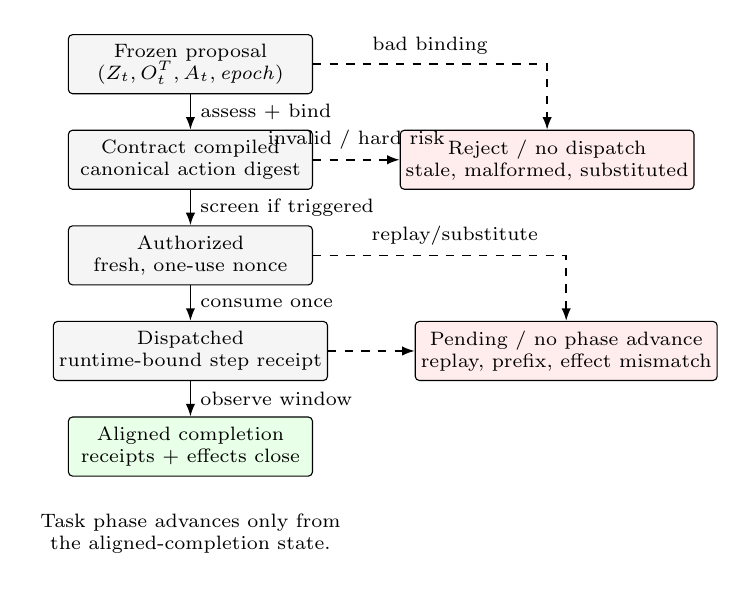
\begin{tikzpicture}[
  font=\scriptsize,
  node distance=4.5mm,
  state/.style={draw,rounded corners=1.5pt,align=center,minimum width=31mm,
                minimum height=7.5mm,fill=gray!8,inner sep=2pt},
  success/.style={state,fill=green!9},
  fail/.style={state,fill=red!7},
  flow/.style={-{Latex[length=1.6mm]},semithick},
  reject/.style={-{Latex[length=1.6mm]},semithick,dashed}
]
\node[state] (proposal) {Frozen proposal\\$(Z_t,O_t^T,A_t,\mathit{epoch})$};
\node[state,below=of proposal] (assessed) {Contract compiled\\canonical action digest};
\node[state,below=of assessed] (authorized) {Authorized\\fresh, one-use nonce};
\node[state,below=of authorized] (dispatched) {Dispatched\\runtime-bound step receipt};
\node[success,below=of dispatched] (closed) {Aligned completion\\receipts + effects close};

\node[fail,right=11mm of assessed] (rejected) {Reject / no dispatch\\stale, malformed, substituted};
\node[fail,right=11mm of dispatched] (pending) {Pending / no phase advance\\replay, prefix, effect mismatch};

\draw[flow] (proposal)--node[right]{assess + bind}(assessed);
\draw[flow] (assessed)--node[right]{screen if triggered}(authorized);
\draw[flow] (authorized)--node[right]{consume once}(dispatched);
\draw[flow] (dispatched)--node[right]{observe window}(closed);
\draw[reject] (proposal.east)-|node[pos=.25,above]{bad binding}(rejected.north);
\draw[reject] (assessed.east)--node[above]{invalid / hard risk}(rejected.west);
\draw[reject] (authorized.east)-|node[pos=.28,above]{replay/substitute}(pending.north);
\draw[reject] (dispatched.east)--(pending.west);

\node[below=3.5mm of closed,align=center,text width=39mm] {
  Task phase advances only from the aligned-completion state.};
\end{tikzpicture}
}
\caption{L2a transaction states.  A triggered L2b screen must qualify between
contract construction and authorization; negative evidence cannot advance the
phase, and a consumed authorization cannot be replayed.}
\label{fig:l2a-transaction}
\end{figure}

\subsection{C3: L2b Bounded Guard Screening}

On every step, the runtime computes the minimum across fourteen joint-side margins.  If the minimum is greater than $0.30$\,rad, the source action takes the fast path: no shadow simulator is invoked.  Otherwise, the runtime identifies the dangerous joint sides and constructs at most two temporary virtual-stop configurations.

Every candidate starts from the same simulator snapshot and executes the same source action for a one-step shadow rollout.  Pre-dispatch eligibility requires exact snapshot restoration, fourteen predicted margins of at least $0.15$\,rad, source-action/guard/restore identity, and a MuJoCo generalized-constraint-force proxy no greater than 10,000.  The runtime selects the weakest eligible uniform guard.  Receipts, realized margins, and prediction error are recorded after dispatch and cannot retroactively qualify a candidate.  If none is eligible, the monitor records a fail-closed task failure without dispatch.

The number ``two'' counts guard configurations, not policy candidates.  This keeps $K=1$ for the VLA and prevents a safety mechanism from being misreported as best-of-$K$ policy improvement.

\subsection{End-to-End Decision Procedure}

For every policy call, the monitor executes the following order.  It first
captures $O_t^T$, advances the trusted FSM, and freezes $Z_t$ before invoking
the policy.  It then receives exactly one $A_t$, constructs the L1 assessment,
and stops if a hard verdict is present.  Otherwise it compiles $C_t$ and, near
a registered joint-side trigger, screens at most two guard configurations from
the same restored snapshot.  A qualifying execution receives a fresh one-use
authorization bound to the episode nonce and current proposal;
each low-level step must match the authorized command and state epoch before
dispatch.  Finally, receipts and effects close the transaction.  A task phase
can advance only after aligned completion; an advisory can only influence the
next policy call.  This order prevents post-action relabeling of $Z_t$, replay
of an old authorization, and use of future outcome as present-time evidence.

\subsection{Failure Semantics}

\system distinguishes four outcomes: \emph{hard reject} for covered physical or integrity failure; \emph{advisory replan} for task-progress uncertainty; \emph{fail-closed no-dispatch} when no safe guard qualifies; and \emph{aligned completion} when the transaction and task evidence both close.  The distinctions are retained in the trace rather than collapsed into task success, allowing the implementation to distinguish safe failure, unsafe success, and utility-preserving executions with severe risk steps.

\section{Implementation and Formal Semantics}
\label{sec:implementation}

\subsection{Runtime Integration}

We implement \system at the consumer/dispatch boundary of the OpenPI $\pi_{0.5}$ LIBERO-Safety runner.  The policy checkpoint, model weights, and action-generation procedure are unchanged.  A trusted-context module manages allowlists and semantic artifacts; a deterministic action-selection module checks frontier and digest consistency; and a runtime wrapper orders policy output, assessment, contract construction, optional guard screening, authorization, dispatch, receipts, and effects.

In the evaluated runner, all policy-generated steps enter this wrapper before the sole \texttt{env.step} boundary.  Thus, complete mediation is conditional on the TCB containing every dispatch path and remaining intact; registered negative tests do not rule out an uninstrumented actuator path in another deployment.

The runner records separate trusted- and policy-observation digests, exact policy-prompt bytes and digest, source and returned action digests, the local assessment, contract and authorization identifiers, step receipts, effect evidence, guard and restore events, joint-side margins, force, and latency.  An action-trace adapter groups actually consumed low-level commands by policy-call index.  It preserves the original policy-chunk digest but never reconstructs an unexecuted tail or uses future reward, success, collision, or observation as present-time evidence.

Action identity is not a hash of raw array memory.  The runtime converts the
flattened action to a finite tuple of Python floats; the proposal also binds its
rank-two shape.  Schema-tagged payloads are key-sorted and encoded as
whitespace-free UTF-8 JSON before SHA-256.  Thus, ``exact'' means equality in
this canonical numeric domain, not equality of array dtype, endianness, or
buffer layout, and not equality of the resulting physical trajectory.

The no-risk path performs no shadow rollout.  The risk path evaluates at most two guard configurations from the same snapshot.  This bounded design makes the screening budget explicit and prevents an unbounded search from hiding in average latency.

\subsection{Reproducibility Bindings}

The frozen evaluation binds OpenPI commit \texttt{15a9616a0094},
LIBERO-Safety commit \texttt{ef0f79b70fc5}, and SABER commit
\texttt{22ad50642a2a}; the artifact manifest records the complete hashes.  The control frequency is
20\,Hz, the policy replans every ten steps, and an episode is capped at 600
steps after ten simulator warm-up steps.  Protocols bind the checkpoint
metadata, environment and policy seeds, rotated arm schedule, source hashes,
and expected output checksums.  The reproducibility record comprises the
freezers, frozen JSON protocols, terminal evidence, negative integrity suite,
Lean sources, and an executable claim-to-evidence audit.  Reported aggregates
are re-derived from frozen traces rather than accepted as prose-transcribed
constants; the audit additionally checks that the corresponding paper tokens
match the recomputed values.

The final runs assign policy inference and EGL simulation to distinct NVIDIA
RTX 6000 Ada Generation GPUs (48\,GiB each; driver 570.133.07).  The policy
receives the \texttt{agentview} and wrist-camera RGB streams, each resized to
$224\!\times\!224$.  Screening latency is measured with a monotonic clock from
the joint-margin read through bounded candidate construction, shadow steps,
snapshot restoration, and candidate selection.  It excludes policy inference
and the subsequently dispatched environment step; it is therefore a
mechanism-specific measurement on this research platform, not end-to-end
control-loop latency.

\subsection{Component Qualification}

The deterministic semantic selector is frozen before the main four-arm study.  On a 160-case qualification corpus, it exactly matches all 160 expected task-frontier outputs.  This result qualifies a privileged benchmark FSM; it does not measure visual perception or open-world generalization.  The analytic local checker and effect observer separately pass frozen finite-corpus gates that exercise supported atoms, malformed or stale objects, and fail-closed behavior.  We use these tests to catch implementation defects, not as a substitute for deployment-distribution safety statistics.

\subsection{Lean Model}

The Lean model defines the four-arm feature switches, \actionblock and assessment identities, execution contracts, authorizations, receipts, effects, and allowed phase transitions.  It proves finite transaction properties rather than physical safety.  The central theorem families establish that:
\begin{itemize}
  \item an authorization binds the same semantic identity and exact final command;
  \item a consumed authorization is unavailable for replay;
  \item every bound receipt uses the same authorization and its applied digest equals its receipt-authorized digest;
  \item unknown effects or an incomplete executed prefix cannot satisfy execution alignment; and
  \item phase advance in an execution-enabled arm requires alignment and contract completion.
\end{itemize}

These theorems make negative states explicit: the model does not permit an unknown effect, partial prefix, or mismatched receipt to become a completed transaction merely because the Python runner continued.  Separately, the Python runtime checks receipt order and binds every applied-step digest to \texttt{authorization.action\_at(i)}.  Appendix~\ref{app:lean} maps paper claims to theorem names.

\subsection{Formal Boundary}

Lean does not parse natural-language intent, choose $Z_t$, prove checker or observer correctness, validate the trusted sensor, or establish that the simulator matches a robot.  A complete refinement proof from the Python serializer and runtime observer to Lean is also future work.  In particular, the current model does not independently bind a receipt's authorized per-step digest to a typed ordered command list; that correspondence is enforced in Python.  The current \texttt{BlockExecutionContract} also does not type the virtual-guard/controller configuration as a separate digest.  We therefore use the phrase \emph{Lean-checked execution transaction semantics}, not \emph{formally verified robot safety}.

\section{Evaluation}
\label{sec:evaluation}

The evaluation follows the preceding security argument.  It first measures
whether an upstream instruction attack reaches the physical-risk endpoint, then
characterizes the final monitor and its stage ablations, and finally tests the
specific enforcement properties claimed by C1--C3.  Three questions guide the
evaluation.
\begin{itemize}
  \item \textbf{RQ1. Attack propagation.}  How often does the frozen SABER
  instruction attack create a new physical-risk transition over a matched clean
  execution?
  \item \textbf{RQ2. System-level outcomes.}  How do \lone, \ltwo, and their
  composition affect task success, the broad risk-transition endpoint, and the
  registered joint-side property?
  \item \textbf{RQ3. Mechanism behavior and cost.}  Do the monitor boundaries
  reach the expected state under targeted semantic and transaction faults, and
  what cost and failure modes does guard screening introduce?
\end{itemize}

The \ltwo arm combines \transactionbinding and \guardscreening, so their
component-specific physical effects are not identifiable from the four-arm
contrast.  Focused transaction cases characterize \ltwoa, while joint-side
measurements and screening latency characterize \ltwob.

\subsection{Experimental Design}

\paragraph{Platform and workload}
The victim is OpenPI $\pi_{0.5}$~\cite{pi05} running on
LIBERO-Safety~\cite{liberosafety2026}.  The policy runs at a 20\,Hz control rate,
returns one $H=10$ source block per call, and receives a new observation after
the block is consumed.  Episodes are capped at 600 steps.  Policy inference and
simulation run on separate NVIDIA RTX 6000 Ada GPUs.

The complete population contains 60 task/initialization base pairs, equally
divided among the benchmark's affordance, human-safety, obstacle-avoidance, and
obstacle-with-human subsets and balanced across three difficulty levels.  Two
independently seeded executions of every pair yield 120 seed-specific evaluation
units.  Initializations are selected without observing outcomes.

The attack workload uses SABER constraint-violation instruction
perturbations~\cite{saber2026}.  One bounded, prompt-only attack record is
generated for each base pair without access to victim outcomes and is frozen
before evaluation.  Both seeded units of a pair use the same record.

\paragraph{Two separate studies}
The \emph{attack-reproduction study} runs one clean and one attacked
unprotected rollout for every unit, for 240 episodes.  Each matched execution
shares the task, initialization, environment seed, and policy seed.  This study
estimates the observed attack success rate (ASR).

The \emph{four-arm study} performs new clean and attacked rollouts for every
unit under \vlaonly, \loneonly, \ltwoonly, and \dual, for
$120\times2\times4=960$ attempts.  \vlaonly is the unchanged runtime baseline,
\loneonly and \ltwoonly are stage ablations, and \dual is the final composed
\system prototype.  Runs for a unit share the initial state and random seeds,
and a counterbalanced arm order reduces schedule effects.  The two studies
share population identities, not rollouts or estimands.

All 960 four-arm attempts produce an outcome record.  Each condition contains
98.96\% valid traces (475/480), short of the registered 100\% all-valid
requirement.  The four-arm results are therefore nonconfirmatory.  Task-success
rates count invalid rows as failures, the broad-risk comparison is a
common-eligible complete-case diagnostic, and joint-side measurements are
valid-trace diagnostics.

\begin{figure*}[t]
\centering
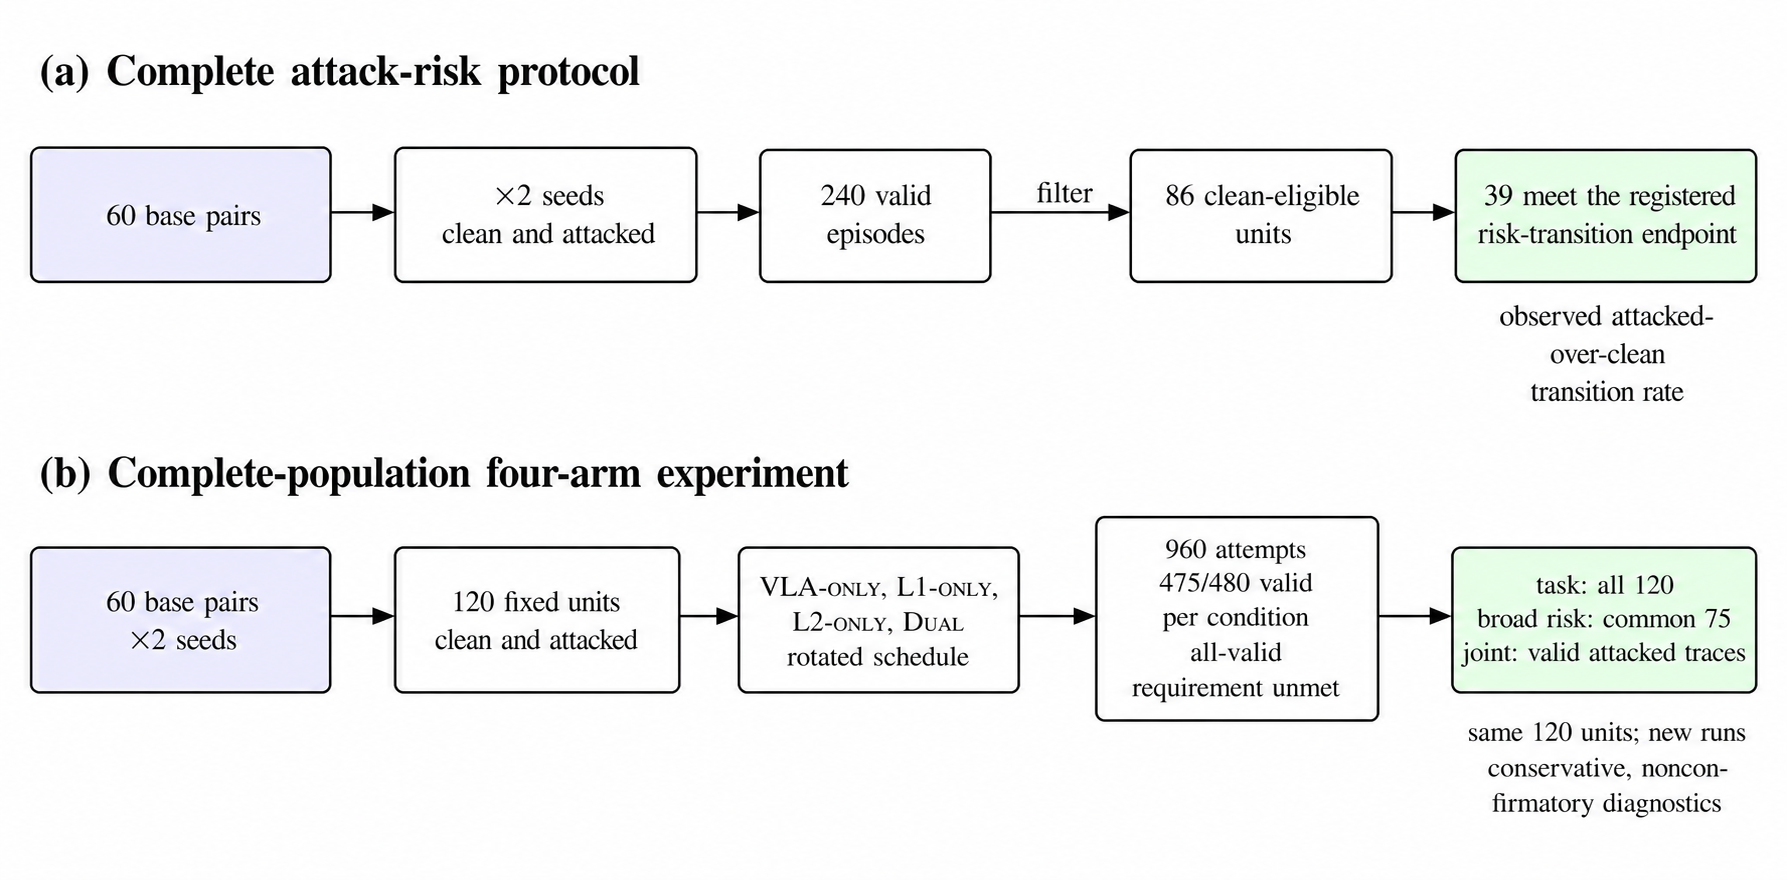
\includegraphics[width=\textwidth]{figures/evaluation_design_raster_v3.png}
\caption{The independent attack reproduction estimates attack propagation.
The separate four-arm study uses new runs over the same 120 population
identities.  Its task-success, broad-risk, and joint-side results use distinct
invalid-trace rules and remain nonconfirmatory.}
\label{fig:evaluation-design}
\end{figure*}

\subsection{Metrics and Counting Rules}

\paragraph{Attack-induced risk transition}
A clean trace is eligible if it is valid, achieves strict task success without a
benchmark cost or collision, and has complete typed constraint-signal and
raw-action coverage.  Clean contact, joint-limit, and force counts need not be
zero.  For an eligible unit with a valid matched attacked trace, a risk
transition occurs when the attacked execution raises the benchmark
cost/collision flag or increases the clean count of robot contacts, joint-limit
steps, or excessive-force steps.  Task failure alone is excluded.

The attack reproduction estimates ASR over its 86 clean-eligible units.  In the
four-arm study, each arm also has a descriptive residual risk-transition rate
over its own clean-eligible units.  Direct cross-arm comparison uses the 75 units
whose clean run is eligible in every arm and whose clean and attacked traces are
valid in every arm.  This common-eligible complete-case cohort gives every arm
the same denominator.  Its rate is a conditional diagnostic, not a
full-population causal effect.

Task-success rates retain all 120 fixed units in every arm, with invalid rows
counted as failures.  Checker rejection is reported among valid traces;
transaction faults are reported over the focused case suite; guard refusal is
reported by valid episode and performed screen.  An invalid trace is not itself
a checker rejection, guard refusal, or observed risk transition.  Percentages
are used for unit- and episode-level outcome rates.  Registered step-level
diagnostics remain counts because no common step-exposure rate was defined.
Paired cross-arm sensitivity tests use exact two-sided McNemar tests on the 75
common-eligible units and carry no confirmatory interpretation.

\subsection{RQ1. SABER Attack Propagation}

All 240 attack-reproduction episodes are valid (100\%).  Among the 86
clean-eligible units, 39 meet the attacked-over-clean risk-transition endpoint.
The observed ASR is therefore 45.35\% (39/86).  This reproduces the SABER
constraint-violation instruction attack on the evaluated OpenPI
$\pi_{0.5}$--LIBERO-Safety path and establishes that the exercised upstream
prompt perturbation can reach the registered physical-risk endpoint.  SABER
serves here as the evaluated Stage-I threat instance; the system objective
continues through the Stage-II execution boundary.

\subsection{RQ2. Final-System and Layer Outcomes}

Table~\ref{tab:task-success} reports the episode-level task-success metric.
Table~\ref{tab:risk-transition} keeps the independent ASR, arm-specific
residual rates, and common-cohort diagnostic visibly separated.

\begin{table}[t]
\centering
\caption{Task-success rates.  Every denominator is the full 120-unit
population; invalid traces count as failures.}
\label{tab:task-success}
\footnotesize
\begin{tabular}{lcc}
\toprule
Arm & Clean & Attacked \\
\midrule
\vlaonly  & 70.83\% (85/120) & 60.83\% (73/120) \\
\loneonly & 65.00\% (78/120) & 53.33\% (64/120) \\
\ltwoonly & 71.67\% (86/120) & 60.83\% (73/120) \\
\dual     & 65.00\% (78/120) & 53.33\% (64/120) \\
\bottomrule
\end{tabular}
\end{table}

\begin{table}[t]
\centering
\caption{Attack-induced risk-transition rates.  The first row is the separate
RQ1 reproduction.  Four-arm native rates use each arm's clean-eligible
denominator; the common column is the matched 75-unit diagnostic.}
\label{tab:risk-transition}
\footnotesize
\setlength{\tabcolsep}{3.5pt}
\begin{tabular}{lcc}
\toprule
Study or arm & Own-cohort rate & Common cohort \\
\midrule
Attack reproduction & 45.35\% (39/86) & N/A \\
\midrule
\vlaonly  & 52.94\% (45/85) & 50.67\% (38/75) \\
\loneonly & 53.85\% (42/78) & 56.00\% (42/75) \\
\ltwoonly & 50.00\% (43/86) & 48.00\% (36/75) \\
\dual     & 55.13\% (43/78) & 57.33\% (43/75) \\
\bottomrule
\end{tabular}
\end{table}

\paragraph{Task success and broad risk}
Under attack, \ltwoonly matches \vlaonly at 60.83\% task success.
\loneonly and \dual each reach 53.33\%.  Relative to \vlaonly, \dual is
5.83 percentage points lower when clean and 7.50 points lower under attack.
The final composed system therefore shows an availability cost in this study.

On the common 75-unit cohort, the broad risk-transition rates are 50.67\%,
56.00\%, 48.00\%, and 57.33\%.  Relative to \vlaonly, the nominal differences
are $+5.33$, $-2.67$, and $+6.67$ percentage points for \loneonly, \ltwoonly,
and \dual.  Exact paired sensitivity tests give $p=0.5034$, $0.6250$, and
$0.3833$, respectively.  No monitored arm provides evidence of a reduction in
the broad endpoint.  This statement remains nonconfirmatory and conditional on
the common-eligible cohort.

\paragraph{L1 (C1) checker behavior and availability}
Among valid \loneonly traces, hard checker rejection occurs in 10.92\% of
clean traces (13/119) and 14.29\% of attacked traces (17/119).  Among the 118
units with valid clean and attacked \loneonly traces, 11 reject in both
conditions, five only under attack, and two only when clean.  The attack-only
rate is 4.76\% (5/105) among clean-accepted complete cases.  All 17 valid
attacked rejections occur before actuator dispatch.

Relative to \vlaonly under attack, 4.17\% of units change from task failure to
success (5/120), while 11.67\% change from success to failure (14/120).  The
net change is $-7.50$ percentage points.  These outcomes match the
checker-relative scope: \lone blocks covered hard findings and imposes a
measurable availability cost; it does not provide complete task semantics.

\paragraph{L2b (C3) joint-side outcome}
The 119 valid attacked \ltwoonly traces and 118 valid attacked \dual traces
form 237 \ltwoenabled traces.  None contains a joint-limit step, giving a
trace-level incidence of 0.00\% (0/237) and a step total of zero.  The
corresponding valid attacked \vlaonly and \loneonly traces record 4,960 and
2,452 joint-limit steps.  This is the positive result targeted by
\guardscreening, within a valid-only registered joint boundary.  The broader
endpoint additionally includes contact, force, cost, and collision; its rate
does not fall for the final composed system.

The RQ2 evidence therefore describes a scoped trade-off.  The targeted
joint-side event is absent from valid attacked \ltwoenabled traces, while
\dual task success is lower than \vlaonly and the broad risk endpoint does not
improve.

\subsection{RQ3. Transaction Behavior and Runtime Cost}

\paragraph{L2a (C2) targeted fault cases}
Targeted tests inject stale context, source-row substitution, replay,
reordering, cross-proposal evidence, incomplete prefixes, missing or unknown
effects, and compromised-sink behavior.  All 69 focused transaction and runner
cases reach their expected state (100\%).  Stale context and malformed binding
reject before dispatch; substitution and reordering fail to match the open
transaction; replay, spliced evidence, and incomplete prefixes cannot close it;
and missing, forbidden, or unknown effects prevent task-phase advance.

The compromised-sink cases expose the TCB boundary.  A sink that changes the
action but reports truthfully produces a receipt mismatch.  A sink that changes
both the action and its evidence is accepted.  Software transaction binding
cannot detect a coordinated lie inside the TCB.

\paragraph{L2b (C3) screening behavior and cost}
Across the 237 valid attacked \ltwoenabled traces, the monitor performs 78,434
screens.  The 95th-percentile screening latency is 23.47\,ms; 0.41\% of screens
exceed 100\,ms (323/78,434), and the maximum is 458.99\,ms.  The registered
maximum-at-most-200\,ms criterion therefore fails, and the prototype has no
hard-real-time guarantee.  These measurements cover the screening interval on
the research simulator, excluding policy inference and real-hardware dispatch.

Across valid attacked \ltwoenabled screens, the maximum post-step observed
generalized-constraint-force proxy is 229.5709, and the maximum
prediction/execution margin error is $2.41\times10^{-5}$\,rad.  The observed
force proxy differs from the predispatch shadow-force candidate gate, so it is
an execution diagnostic rather than validation of that gate.

Across valid clean and attacked \ltwoenabled traces, five episodes contain one
guard refusal each.  This is 1.05\% of valid \ltwoenabled episodes (5/474) and
0.0034\% of performed screens (5/146,397).  Every refusal has the registered
no-bounded-force-feasible-guard-candidate reason and ends without actuator
dispatch.  These results qualify the exercised simulator path; they do not
validate a dynamics model for a physical robot.

\paragraph{Summary}
RQ1 reproduces SABER with a 45.35\% attacked-over-clean ASR.  RQ2 finds no
broad risk or task-success improvement for the final composed system, while
valid attacked \ltwoenabled traces show the targeted zero-joint-limit
diagnostic.  RQ3 shows that all 69 focused cases reach their expected state,
including the compromised-sink limitation, and that guard screening has a
measured long-latency tail.  Every conclusion remains bounded by the registered
checker, TCB, guard, simulator, attack family, and trace-validity rules.

\section{Security Analysis and Discussion}
\label{sec:discussion}

\subsection{What the Evidence Shows}

The two studies answer different questions.  The independent attack
reproduction shows that a bounded SABER instruction perturbation can propagate
through an unprotected \vla to the registered physical-risk endpoint.  Its
observed ASR is 45.35\% among 86 clean-eligible units (39/86).  The four-arm
study then characterizes the final \system prototype and its stage ablations at
the consumer boundary.  It shows predispatch rejection for the covered C1 findings, the
expected response to the exercised C2 transaction faults, and 0.00\%
trace-level joint-limit incidence across 237 valid attacked \ltwoenabled traces.

The system-level result does not show a broad safety improvement.  On the common
75-unit cohort, the broad risk-transition rates are 50.67\%, 56.00\%, 48.00\%,
and 57.33\%, and no monitored arm provides evidence of a reduction relative to
\vlaonly.  Under attack, \dual task success is 53.33\%, compared with 60.83\%
for \vlaonly.  Moreover, each condition is 98.96\% valid against a registered
100\% requirement, so the four-arm results cannot support a confirmatory
overall-effect claim.  The
paper therefore treats the C1, C2, and joint-side observations as bounded
property evidence, not as proof that \system makes the robot generally safer.

\subsection{Why Local Properties Do Not Imply End-to-End Safety}

The evaluation illustrates why the three components must be interpreted
separately.  \lone and \ltwo protect different alignment stages; \ltwoa and
\ltwob supply distinct evidence within the second stage.  \taskassessment
enforces a declared checker vocabulary against an
independently anchored task state.  It can stop a covered hard finding before
dispatch, but an incomplete checker can reject useful actions or miss hazards
outside its predicates.  The observed task-completion loss is therefore not an
incidental reporting detail; it is the availability cost of the current checker
boundary.

\transactionbinding answers a different question.  It determines whether
execution evidence still refers to the proposal that received permission.  It prevents a covered
substitution or replay from being mistaken for aligned execution, but a faithfully
executed authorized action can still be physically undesirable.  It also cannot
detect a trusted sink that changes both the action and the evidence it reports.

\guardscreening targets one registered joint-side condition.  Its zero
joint-limit observation in valid attacked \ltwoenabled traces is consistent with that
local goal, while the broader endpoint still includes contact, force,
cost/collision, and other pathways not eliminated by the joint guard.  Changing
the guard/controller configuration can also alter task progress even though the
policy-emitted source action remains fixed.  Consequently, source-action
integrity, local constraint enforcement, task success, and broad physical risk
are related but non-equivalent properties.

\subsection{Dependence on the TCB and Registered Models}

The authorization claim depends on a task and observation path that is
independent of the attacked policy view.  The evaluated prototype realizes this
path with privileged simulator task state and geometry.  A deployable camera-only
or sensor-based trusted path would need its own integrity and accuracy evidence;
errors before the trusted split are outside the current guarantee.

The execution claim assumes complete mediation, protected monitor state, and
truthful receipts and actuator feedback.  Contract binding ranges only over the
effects the contract declares, so omitted hazards remain uncovered.  Likewise,
the checker-relative claim depends on the registered predicates.  Unknown
inputs trigger configured fail-closed handling; no general semantic judgment
follows.

The guard evidence uses the LIBERO/robosuite dynamics
~\cite{robosuite2020} and the same simulator model for shadow screening and
post-restore execution.  It qualifies snapshot restoration and the registered
joint-margin and force measurements in that environment.  It does not establish
model fidelity, robustness to real sensor noise, or physical-robot safety.  The
Lean model is narrower still: it checks selected abstract authorization,
ordered-action, evidence, and phase relations, not the prototype-to-model
refinement or continuous dynamics.

\subsection{Statistical and Empirical Limitations}

The four-arm study produced 1.04\% invalid rows in each condition (5/480)
against a registered zero-invalid requirement.  Task counts retain all 120 units with
invalid runs counted as failures, but the broad-risk comparison uses 75 units
that are eligible and valid in every arm.  That common cohort enables a matched
comparison with a shared denominator; it is not a full-population causal
estimate.  The zero joint-limit result similarly covers only the 237 valid
attacked \ltwoenabled traces and cannot be extended to invalid runs.

The empirical scope contains one $\pi_{0.5}$ checkpoint, one simulator
benchmark, and one frozen SABER instruction-attack family.  Defense-aware
adaptive attacks are not evaluated, although recent work shows their importance
~\cite{adaptivesecond2026}.  Other visual or post-inference channels belong to
the threat model but are represented here only by focused transaction cases, not
full end-to-end attack campaigns.  Finally, the 458.99\,ms maximum screening
latency violates the registered 200\,ms bound, so the prototype has no
hard-real-time guarantee.  Broader attack families, trusted perception, more
complete physical predicates, and real-robot evaluation are necessary before
claiming wider protection.

\section{Related Work}
\label{sec:related}

Related work is organized around the two alignment stages.  The first question
is where task authority comes from and how it reaches an online \actionblock.
The second is how far the resulting evidence follows that block toward physical
execution.  Section~\ref{sec:background} gives the capability-level comparison;
the discussion below explains the corresponding mechanisms and claim
boundaries.

\subsection{VLA Attacks, Safety, and Candidate Verification}

SABER uses bounded instruction edits to stress-test \vla policies
~\cite{saber2026}.  FreezeVLA studies action-freezing attacks against \vla
models, while BadRobot and RoboPAIR study jailbreaks of embodied agents and
LLM-controlled robots~\cite{freezevla2025,badrobot2025,robopair2025}.  A recent
survey organizes this broader space by multimodal attack surface, physical
effect, real-time constraint, and long-horizon propagation~\cite{vlasafety2026}.
These works establish that corrupt context can alter embodied behavior; RQ1
measures how often one such attack reaches a paired physical-risk endpoint in the
studied action-only path.

LIBERO-Safety, SafeVLA-Bench, and ForesightSafety-VLA separate task completion
from safety outcomes~\cite{liberosafety2026,safevlabench2026,
foresightsafety2026}.  SafeVLA integrates constraints during policy training,
and SAFE learns rollout-failure detection~\cite{safevla2025,safe2025}.  These
approaches modify or train the policy, whereas \system leaves the checkpoint and
policy interface unchanged and mediates its output at runtime.

SEAL samples action sequences, predicts outcomes, and selects against a
reasoning \vla's textual plan~\cite{sealvla2026}.  CoVer learns a contrastive
instruction--observation--action verifier and scales across rephrased
instructions and action candidates~\cite{covervla2026}.  Their authority comes
from a policy plan or learned candidate score.  \system instead assesses one
source block against independently anchored task state and carries that same
proposal into dispatch and effect evidence.  The approaches are complementary.
Candidate quality and execution integrity are different claims.

\subsection{Trusted Inputs and Digital-Agent Execution}

An agent-security SoK maps the broader attack-and-defense landscape
~\cite{agenticsok2026}.  StruQ separates trusted and untrusted query fields, and
SecAlign uses preference optimization for prompt-injection defense
~\cite{struq2025,secalign2025}.  Studies of deployed plugins and tool-using
agents show attacks through conversation history, tool metadata, source
ordering, and cross-tool flow~\cite{webplugins2026,toolhijacker2026,
obliinjection2026,lesdissonances2026}.  This line of work motivates separating
trusted authority from mutable model context.

CaMeL derives protected control and data flow from a trusted query, while ACE
derives trusted abstract plans and enforces data and capability barriers
~\cite{camel2026,ace2026}.  IsolateGPT, SAGA, and automated permission systems
add application isolation, agent identity, and data-access control
~\cite{isolategpt2025,saga2026,agentpermissions2026}.  AttriGuard causally
attributes tool calls, and MATE learns a policy-conditioned mobile-agent
trajectory auditor~\cite{attriguard2026,mate2026}.  Their protected objects are
digital control flows, calls, identities, permissions, or mobile-agent
trajectories.  \system applies the trusted-authority principle to a high-rate
continuous actuator transaction and follows the online source block beyond the
digital decision point.

\subsection{CPS Integrity, Robot Attestation, and Shielding}

DIAT addresses malicious modification of generated or processed data through
control-flow-backed attestation~\cite{diat2019}; CFA+ detects or prevents
control-flow hijacking~\cite{cfaplus2024}; and ARTO protects control and data
flow in real-time CPS~\cite{arto2026}.  SCAPHY correlates industrial-control
program behavior with physical behavior~\cite{scaphy2023}.  TAT addresses
robot-motion manipulation using motion-event and joint evidence
~\cite{tat2026}.  These systems begin from a protected program, execution, or
reference motion.  The protected object in \system is a newly generated
continuous block whose task-relative assessment must be connected to later
execution.

VLMPC predicts action-conditioned frames for candidate action sequences, and
SafetyChance calibrates predicted safety for image-controlled autonomy
~\cite{vlmpc2024,safetychance2024}.  Measurement-robust control barrier
functions and continuous-space shields enforce defined safety sets
~\cite{measurementrobustcbf2021,realizableshields2025}.  These methods motivate
state-conditioned qualification.  In \system, that qualification is one part of
a larger evidence lifecycle: it names both the fixed source action and the
controller configuration used to realize it, and remains limited to the
registered joint boundary.

Classic protection design requires complete mediation and fail-safe defaults
~\cite{saltzer1975}, while execution-monitoring theory characterizes properties
enforceable over event prefixes~\cite{schneider2000}.  \system applies these
principles to proposal, dispatch, receipt, effect, and phase events.  Lean checks
selected abstract transaction relations; sensing, checker coverage, and dynamics
remain explicit TCB or empirical assumptions.

Taken together, prior systems protect upstream authority, candidate selection,
downstream execution integrity, or local physical constraints.  The composition
developed here is a single lifecycle that binds independent task authority to
the exact generated block, carries the same proposal through ordered execution
evidence, and records its state-conditioned realization.

\FloatBarrier
\section{Conclusion}

\system is a cross-layer reference monitor for two alignment stages at the
action-only \vla boundary.  \lone binds trusted task intent to the exact online
\actionblock through a checker-relative assessment.  \ltwo then binds the
authorized block to execution: \ltwoa preserves proposal identity through a
one-use ordered transaction and its evidence, while \ltwob qualifies the same
source action at the registered joint boundary.  The
\proofaligned property composes these obligations, and Lean checks
selected abstract transaction and phase relations.

The independent SABER reproduction measures a 45.35\% attack-induced
risk-transition rate among 86 clean-eligible units (39/86).  The separate
120-unit four-arm study produces 960 episode attempts, with 98.96\% valid traces
in each condition (475/480).  Its registered all-valid requirement is unmet, so
the system comparisons remain nonconfirmatory.  On the common 75-unit cohort,
the risk-transition rates for \vlaonly, \loneonly, \ltwoonly, and \dual are
50.67\%, 56.00\%, 48.00\%, and 57.33\%; no paired contrast provides evidence of
a broad reduction.  Under attack, task success is 60.83\% for \vlaonly and
53.33\% for \dual.  The targeted joint-side observation is narrower: 0.00\%
of the 237 valid attacked \ltwoenabled traces contain a joint-limit step (0/237), while
the valid attacked \vlaonly and \loneonly traces record 4,960 and 2,452 such
steps.

The evidence is checker-relative, simulator-bound, and limited to the stated
TCB, attack family, and valid traces.  It does not establish a broad
robot-safety improvement or hard-real-time guarantee.

\section*{Generative-AI Disclosure}
OpenAI Codex desktop app (GPT-5 model family; accessed August 2026) assisted across all manuscript
sections with drafting and editing and generated the LaTeX/TikZ diagrams for
Figs.~2--3 and raster artwork for Figs.~1 and~4 from author-supplied designs,
protocols, results, and claim boundaries.  Its role was limited to manuscript
and diagram production.  The
authors conducted the experiments, determined the reported outcomes, reviewed
the generated material, and remain responsible for every claim, number,
citation, and artifact.

\section*{Ethics Considerations}
The study is simulator-only: every attack, benchmark agent, and contact in
\texttt{human\_safety} is synthetic.  Its data consist of benchmark task
instances, simulator traces, and system logs.  The attack target is the
OpenPI $\pi_{0.5}$ model evaluated on the LIBERO-Safety
benchmark~\cite{pi05,liberosafety2026}.  The paper retains every
fixed evaluation unit, explicit error record, residual risk transition, and
frozen audit record.  The prototype's intended use is supervised research on
action-boundary monitoring.


\bibliographystyle{IEEEtran}
\bibliography{paper}

\appendix
\section{Supplementary Security and Reproducibility Details}

\subsection{Lean Claim Map}
\label{app:lean}

\begingroup
\scriptsize\sloppy
Exact theorem names in \texttt{ProofAlign.SemanticIntegrityCore}:
\nolinkurl{authorization_binds_semantic_identity},
\nolinkurl{authorization_binds_exact_final_command};
\nolinkurl{consumed_authorization_not_available};
\nolinkurl{every_bound_receipt_uses_same_authorization},
\nolinkurl{every_bound_receipt_applies_exact_action};
\nolinkurl{unknown_effects_block_execution_alignment},
\nolinkurl{incomplete_prefix_blocks_execution_alignment};
\nolinkurl{execution_enabled_phase_advance_requires_alignment}, and
\nolinkurl{phase_advance_requires_contract_completion}.
\endgroup

Despite its historical name,
\nolinkurl{every_bound_receipt_applies_exact_action} proves only equality of a
receipt's applied and authorized digests; Python-to-Lean refinement to the
ordered step list is outside scope.


\end{document}
